%%%%%%%%%%%%%%%%%%%%%%%%%%%%%%%%%%%%%%%%%
% Simple Sectioned Essay Template
% LaTeX Template
%
% This template has been downloaded from:
% http://www.latextemplates.com
%
% Note:
% The \lipsum[#] commands throughout this template generate dummy text
% to fill the template out. These commands should all be removed when 
% writing essay content.
%
%%%%%%%%%%%%%%%%%%%%%%%%%%%%%%%%%%%%%%%%%

%----------------------------------------------------------------------------------------
% PACKAGES AND OTHER DOCUMENT CONFIGURATIONS
%----------------------------------------------------------------------------------------

\documentclass[12pt]{article} % Default font size is 12pt, it can be changed here
\usepackage[utf8]{inputenc} % utf8 support
\usepackage[T1]{fontenc}

\usepackage{geometry} % Required to change the page size to A4
\geometry{a4paper} % Set the page size to be A4 as opposed to the default US Letter

\usepackage{graphicx} % Required for including pictures

% \usepackage{float} % Allows putting an [H] in \begin{figure} to specify the exact location of the figure
\usepackage{wrapfig} % Allows in-line images such as the example fish picture

\usepackage[style=numeric, backend=biber, sorting=none]{biblatex}
\bibliography{kilgarvan.bib}

\linespread{1.2} % Line spacing

%\setlength\parindent{0pt} % Uncomment to remove all indentation from paragraphs

\graphicspath{{./img/}} % Specifies the directory where pictures are stored

\newlength{\wideitemsep}
\setlength{\wideitemsep}{.5\itemsep}
\addtolength{\wideitemsep}{-7pt}
\let\olditem\item
\renewcommand{\item}{\setlength{\itemsep}{\wideitemsep}\olditem}

\begin{document}

%----------------------------------------------------------------------------------------
% TITLE PAGE
%----------------------------------------------------------------------------------------

\begin{titlepage}
  \newcommand{\HRule}{\rule{\linewidth}{0.5mm}} % Defines a new command for the horizontal lines, change thickness here

  \center % Center everything on the page

  \textsc{\LARGE University College Cork}\\[1.5cm] % Name of your university/college
  \textsc{\Large Wind Energy}\\[0.5cm] % Major heading such as course name
  % \textsc{\large Minor Heading}\\[0.5cm] % Minor heading such as course title

  \HRule \\[0.4cm]
  { \huge Kilgarvan Wind Farm Visit 28-10-2015}\\[0.5cm] % Title of your document
  \HRule \\[1.5cm]

  \begin{minipage}{0.4\textwidth}
  \begin{flushleft} \large
  \emph{Author:} Peter \textsc{Armstrong} \\% Your name 
  \emph{Student ID:} 115224113
  \end{flushleft}
  \end{minipage}
  ~
  \begin{minipage}{0.4\textwidth}
  \begin{flushright} \large
  % \emph{Supervisor:} \\
  % Dr. James \textsc{Smith} % Supervisor's Name
  \end{flushright}
  \end{minipage}\\[4cm]

  {\large \today}\\[3cm] % Date, change the \today to a set date if you want to be precise

  \vfill % Fill the rest of the page with whitespace

% itemize changes
\newlength{\wideitemsep}
\setlength{\wideitemsep}{.5\itemsep}
\addtolength{\wideitemsep}{-7pt}
\let\olditem\item
\renewcommand{\item}{\setlength{\itemsep}{\wideitemsep}\olditem}

\end{titlepage}

%----------------------------------------------------------------------------------------
% TABLE OF CONTENTS
%----------------------------------------------------------------------------------------

% \tableofcontents % Include a table of contents

% \newpage % Begins the essay on a new page instead of on the same page as the table of contents 

%----------------------------------------------------------------------------------------
% INTRODUCTION
%----------------------------------------------------------------------------------------

\section{Site Description} % Major section

The Kilgarvan wind farms are situated on the western side of the Derrynasaggart mountains, Co. Kerry. In the area, there is a cluster of five wind farms. This group of wind farms have been built over the last 10 years.

  \begin{center}
    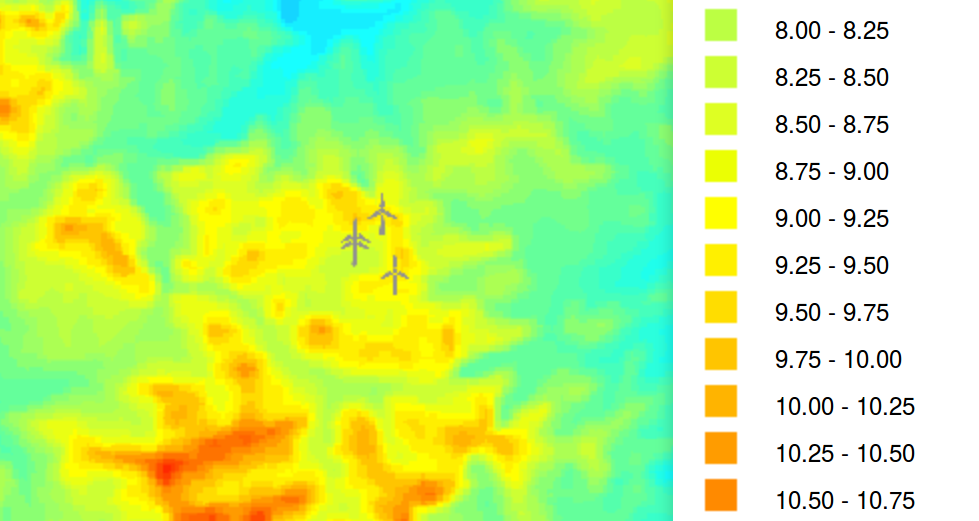
\includegraphics[width=1\textwidth]{seai_wind_atlas_kilgarvan}
  \end{center}
  \caption{Wind speed at 75m - SEAI Wind Atlas - Kilgarvan Area}

According to the SEAI Wind Atlas \cite{seai_atlas}, the area has average wind speeds at 75m height of 8 - 10 ms^-1.

% TODO: Something about wind reliability - weibull

The terrain is flat/not flat - based on what criteria.


\subsection{Access Route}
Access to Kilgarvan windfarm is off the N22. 

The first bit of electricity infrastructure visible is an Eirgrid/ESB operated substation just off the main road. This substation connects directly to the 110kV grid.

The wind farms are situated on the western side of the Derrynasaggart mountains. An access road winds from the Nxxx to the site. The road passes through both rocky and bog areas. Some cutting away of bog and rock was necessary to build the road. The road has a gentle incline and wide turns. Turbines were transported to the site in large sections on this road so it has a gentle incline and wide turns.
% reference for transporting turbine sections
The area on the lee side of the hills is forested. Although the land is owned by the wind farm operator, Brookfield, the forestry is managed by Caoilte.


% research building roads through bogs



\section{Technology Description}
% TODO: Main kilgarvan site ?? Proper names?
There are two types of wind turbine installed on the site that was visited. The Vestas V90 is a 3MW turbine. The blades are made from lightweight carbon fibre and glass fibre composite materials. The nacelle and tower are also designed to reduce weight. The light weight reduces transportation, installation and foundation costs \cite{v90-3.0}. The V90 has a rotor diameter of 90m.
Vestas \cite{v90-3.0} describe the V90 as 'a great choice for high- and medium-wind sites with high turbulence'. 
The V90 can be used with a variety of different tower heights, but at Kilgarvan it is mounted on a 75m tower. The V90 was originally designed for offshore use. The turbines at Kilgarvan were the first V90 turbines installed onshore.
There are XX Vestas V90 turbines on the site and they are approximately 8 years old.

The other turbine on the site is the Nordex N90. This is a 2.5MW turbine with a 90m rotor diameter. It has similar design specifications as the Vestas V90. Nordex \cite{n90} describe the N-90 as 'As an all-round turbine ... (that) can be deployed at strong-wind sites'.

Both turbines meet the IEC-1A certification. Turbines with this certification are designed for average wind speeds of 10m/s with extreme 50 year gusts of 50m/s \cite{burton_wind_2001}. The A certification means these turbines are suitable for use in areas of high turbulence.

The Noredex turbine uses an electrical pitch control system. Each turbine has battery backup for the pitch control system.

The Vestas machines use a hydraulic pitch system that does not require battery backup.

The blades on the Vestas machines appear to be swept back significantly. The Nordex blades appear straighter.

\begin{center}
  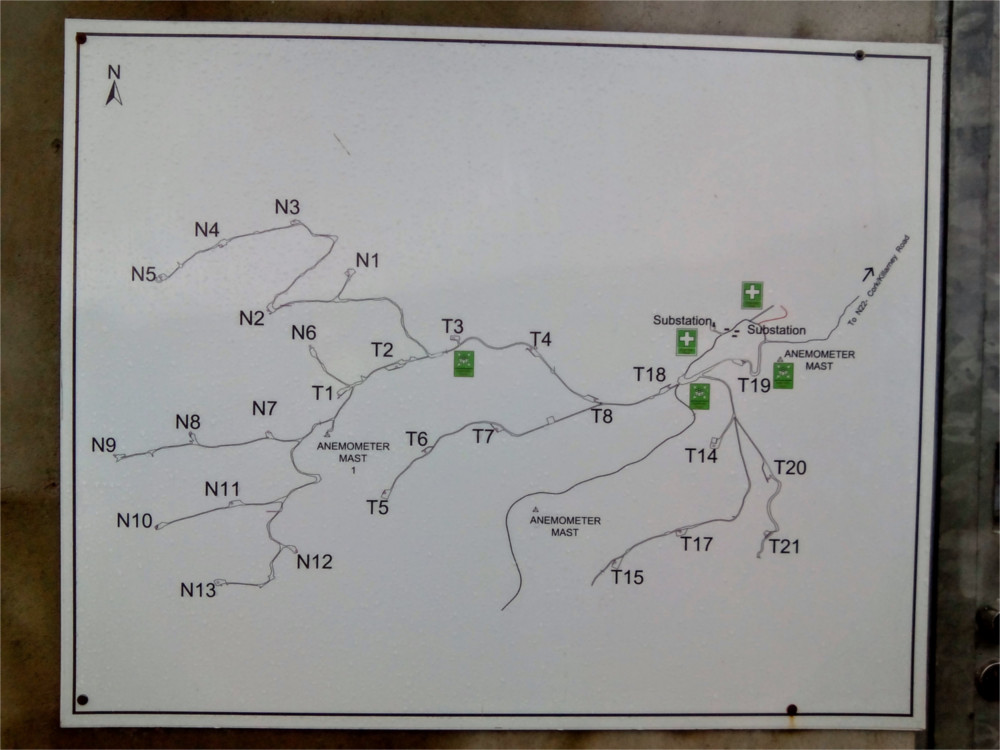
\includegraphics[width=1\textwidth]{kilgarvan_layout}
\end{center}
\caption{Layout of the wind farm. N indicates a Nordex turbine, T indicates a Vestas machine}

Each turbine has an access door at the base of the tower. Inside, there is a voltage converter, turbine control system and a ladder and lift to access the nacelle.

\subsection{Maintenance Requirements}
\paragraph{Planned Maintenance:}
Type 3 maintenance was recently completed on the Nordex machines at the Kilgarvan site. Technicians from Nordex come on site to do the maintenance. Type 3 maintenance involves replacing the battery backups and tightening every bold in the turbine. During maintenance, the turbine must be stopped. Type 3 maintenance takes one week and the turbine will be down for between 8-10 hours per day.

\paragraph{Unplanned Maintenance:} 
Another unexp

\subsection{Electrical Infrastructure}
The turbines generate electricity at 1000V. The voltage is stepped up to 20kV at the bottom of the turbine where it is connected to the local on site grid. The voltage is stepped up to 110kV at the Brookfield operated substation at the top of the site.

\section{Operations and Conditions}


\subsection{The day we visited}
The wind speeds on the day of the visit were very variable. The average wind speed was 10m/s but it varied from 6m/s - 13m/s. The pitch of the turbine blades was constantly changing as the automatic control system attempted to get the maximum amount of power from the variable winds.
% TODO: Other name?
The Ray, one of the Brookfield engineers, estimated the turbine was operating at around 75\% capacity due to the variable winds

At the time of the visit, all of the power being generated was being accepted by the grid. This is the usual scenario, as wind, as a renewable source, is higher in the merit order. %TODO: reference merit order.
% TODO: Explain what curtailment means better
From time to time, the grid managers will reject some wind generated power. This may be needed to ensure grid stability. This scenario is known as curtailment.

Ray is a Brookfield engineer who operates a nearby 100MW farm.
He expected higher, more consistent winds that evening. Due to the stronger winds and lower loads expected at night, Ray expected production from his farm to be curtailed to 75MW that evening. As his farm has a non-firm connection, this means there would be no compensation for the curtailment.

\subsection{A day in the life of a wind farmer}
Ray spoke about his work as an engineer on a wind farm. The work varies and there is no typical day. Public relations are an important aspect of his job. The public are permitted to access the lands around the turbines and the engineers will often meet with them and shoot the shit.
% TODO: remove shoot the shit.
Ray's farm is in a Special Area of Conservation and is a know habitat for some kind of bird.
Wind turbines are known to strike birds from time to time and the Environmental protection agency check the area with sniffer dogs to see if there is any protected birds nesting nearby. If a nest is found near a turbine, that turbine must be shut down.


\section{Conclusion}
Wind farming is a business.
Successful, large companies investing in it.


%----------------------------------------------------------------------------------------
% BIBLIOGRAPHY
%----------------------------------------------------------------------------------------
\printbibliography

%----------------------------------------------------------------------------------------

\end{document}